\chapter{List of Publications} \label{appendix:publications}

    \section{Journal Publications}
    	\subsection{Published}
    		\begin{enumerate}
    			\item \textbf{Parag Bhattacharya}, Monmoyuri Baruah, \textit{``Supersoft X-ray Sources: A Review Study''}, Journal of Applied \& Fundamental Sciences, ISSN 2395-5554 (Print), 2395-5562 (Online), vol. 3 no. 2 (June 2017), Indexing: UGC Approved list (at the time of publication). \label{paper-jafs}
    			
    			\item \textbf{Parag Bhattacharya}, Bansy M. Lyngdoh, Jessica I. Nongrum, Ranjeev Misra and Monmoyuri Baruah, \textit{``A Python-based tool for spectral line identification in RGS spectra from XMM-Newton''}, ADBU Journal of Engineering \& Technology, ISSN: 2348-7305, vol. 9 no. 2 (December 2020), Indexing: UGC-CARE list (at the time of publication). \label{paper-ajet}
    			
    			\item Rabindra Mahato, \textbf{Parag Bhattacharya}, Monmoyuri Baruah, \textit{``A Study of ISM in the Line of Sight of NS Transient LMXB MXB 1659-298''}, Galaxies, ISSN: 2075-4434, vol. 12 no. 4 (July 2024), Indexing: Scopus, ESCI (Web of Science). \label{paper-galaxies}
    		\end{enumerate}
    	
%    	\subsection{Accepted for Publication}
%    		\begin{enumerate}
%    			\item Rabindra Mahato, \textbf{Parag Bhattacharya}, Monmoyuri Baruah, \textit{``A Study of ISM in the Line of Sight of NS Transient LMXB MXB 1659-298''}, Galaxies, ISSN: 2075-4434 (Accepted on 17 July 2024), Indexing: Scopus, ESCI (Web of Science).
%    		\end{enumerate}
    		
    	\subsection{Communicated to Journal}
    		\begin{enumerate}
    			\item \textbf{Parag Bhattacharya}, Rabindra Mahato, Ranjeev Misra and Monmoyuri Baruah, \textit{``Multi-Observatory Spectral Analysis of the Supersoft X-ray Continuum of RX J0925.7-4758''}, Pramana: Journal of Physics, ISSN: 0973-7111 (Communicated on \textit{30 April 2024}, revised on \textit{30 September 2024}), Indexing: Scopus, UGC-CARE list. \label{paper-pram}
    		\end{enumerate}
    
    \section{Conference Presentation}
        \begin{enumerate}
            \item Parag Bhattacharya, Monmoyuri Baruah and Ranjeev Misra, \textit{``A continuum spectral model for RX J0925.7-4758 using ASCA observations''}, 2$^{\text{nd}}$ national conference on Trends in Modern Physics 2020 (TiMP 2020), Assam Don Bosco University, Sonapur, Assam.
            
            \item Parag Bhattacharya, Flossie B. F. C. Marak and Monmoyuri Baruah, \textit{``Comparative Study of the H$\beta$ and He$I$ 4922\AA\ Absorption Lines in the Synthetic Spectra of O-Type Sub-Dwarf Stars''}, North-East Meet of Astronomers 2019 (NEMA-5), Tezpur University, Tezpur, Assam.
            
            \item Parag Bhattacharya, Washim Akram and Monmoyuri Baruah, \textit{``Theoretical Modelling of Stellar Atmospheres using TLUSTY/SYNSPEC''}, North-East Meet of Astronomers 2018 (NEMA-4), Assam University, Silchar, Assam.
            
            \item Parag Bhattacharya, Mizanur Rahman and Monmoyuri Baruah, \textit{``Spectral Fitting of the supersoft X-ray sources RXJ0925.7-4758''}, North-East Meet of Astronomers 2017 (NEMA-3), St. Anthony's College, Shillong, Meghalaya.
            
            \item Parag Bhattacharya, and Monmoyuri Baruah, \textit{``Spectral Fitting of Supersoft X-ray Sources''}, North-East Meet of Astronomers 2016 (NEMA-2), Tezpur University, Tezpur, Assam.
        \end{enumerate}
        
    \newpage
	\begin{landscape}
	\begin{figure*}[htb!]
		\centering
		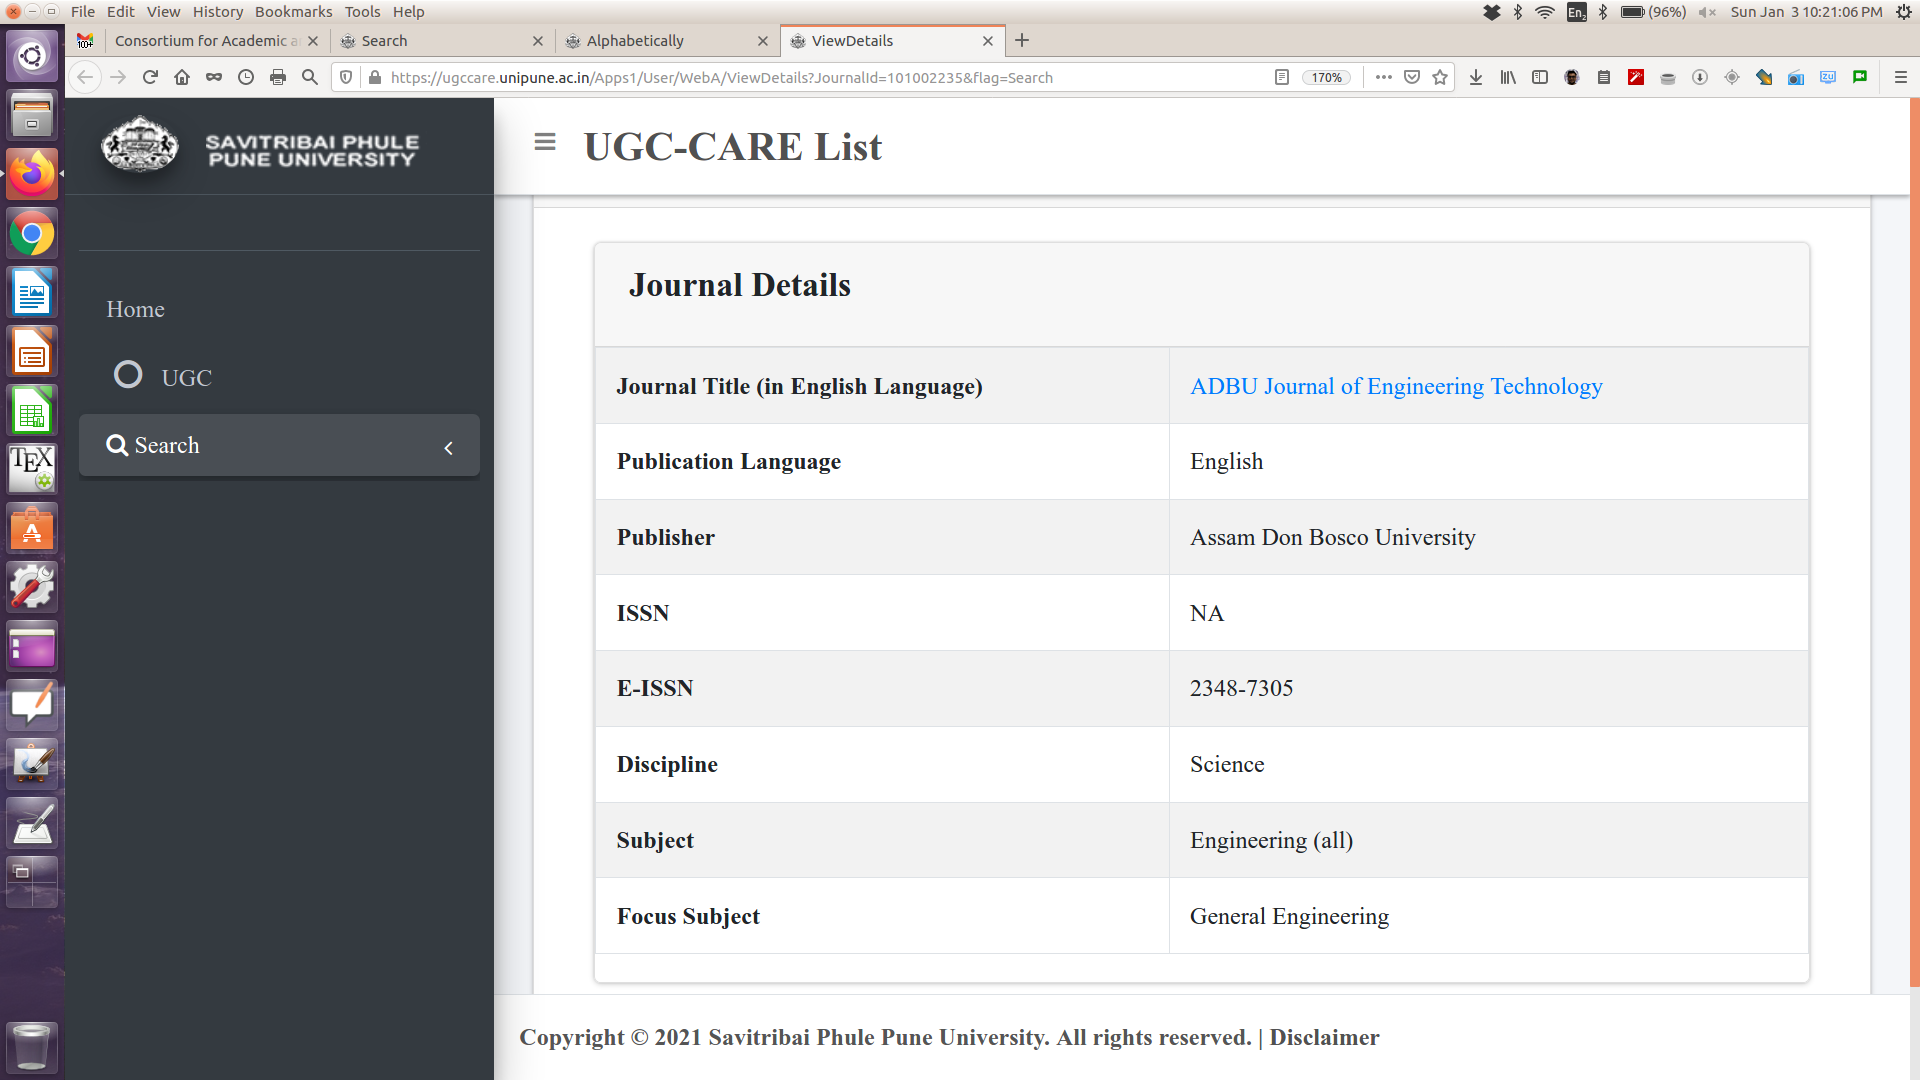
\includegraphics[width=22cm]{ugc-ajet}
		\caption*{Screenshot taken by self, displaying the inclusion of ADBU Journal of Engineering \& Technology (AJET) in UGC-CARE List at the time of publication of paper no. \ref{paper-ajet}.}
	\end{figure*}
	\end{landscape}
        
	\newpage
	\begin{landscape}
	\begin{figure*}[htb!]
		\centering
		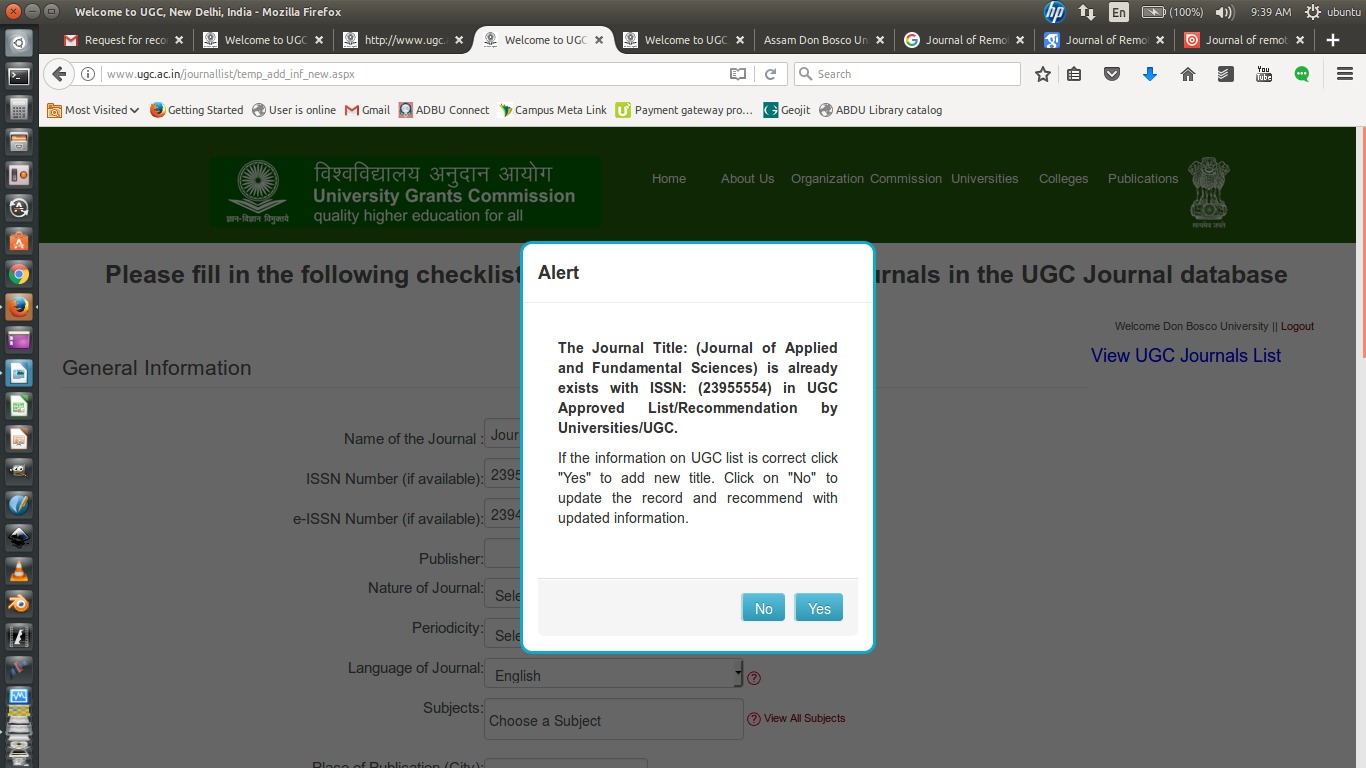
\includegraphics[width=22cm]{ugc-jafs}
		\caption*{Screenshot provided by Dr. Samrat Dey, former Editor-in-Chief of Journal of Applied \& Fundamental Sciences (JAFS), displaying the inclusion of JAFS in UGC Approved List at the time of publication of paper no. \ref{paper-jafs}.}
	\end{figure*}
	\end{landscape}